\appendix
\section{Minimal-RL Training Details}
\label{app: minimal_rl_training_details}
We mainly follow the Minimal-RL recipe~\citep{xiong2025minimalist} in our experiments to ensure a fair comparison among different rollout sampling strategies. Specifically, we set a series of hyperparameters as in \cref{tab: hyperparameter}:

\begin{table}[h!]
\centering
% \resizebox{\textwidth}{!}{%
\begin{tabular}{@{}cc@{}}
\toprule
Hyperparameter                                 & Value(s)        \\ 
\midrule
\multicolumn{1}{c}{Training Batch Size}      & \multicolumn{1}{c}{1024} \\ 
\multicolumn{1}{c}{Max Prompt Length}        & \multicolumn{1}{c}{1024} \\ 
\multicolumn{1}{c}{Max Response Length}      & \multicolumn{1}{c}{3072} \\ 
\multicolumn{1}{c}{Mini Batch Size}          & \multicolumn{1}{c}{256}  \\ 
\multicolumn{1}{c}{Micro Batch Size Per GPU} & \multicolumn{1}{c}{4}    \\ 
\multicolumn{1}{c}{Learning Rate}            & \multicolumn{1}{c}{$10^{-6}$} \\ 
\bottomrule
\end{tabular}%
% }
\caption{Hyperparameter Setup for Running Minimal-RL recipe. }
\label{tab: hyperparameter}
\end{table}

\section{Off-policy Issue and Truncated Importance Sampling Correction}
\label{sec:off-policy}
\subsection{Sampling Techniques Can Introduce Off-Policy Issue}
\label{subsec:temperature-sampling}
One subtle yet troublesome drawback of reinforcement learning with sampling techniques is that it simultaneously introduces the \emph{off-policy} problem: there is a gap between the behavior policy (used for sampling) and the target policy (being optimized and parametrized by $\theta$). This might introduce instability to the training and cause it to fail (See example training of RLVR with EAD \cref{fig:optim_failure_for_as_offpolicy}).

\begin{figure}[h!]
    \centering
    \begin{subfigure}[b]{0.26\textwidth}
    \centering
    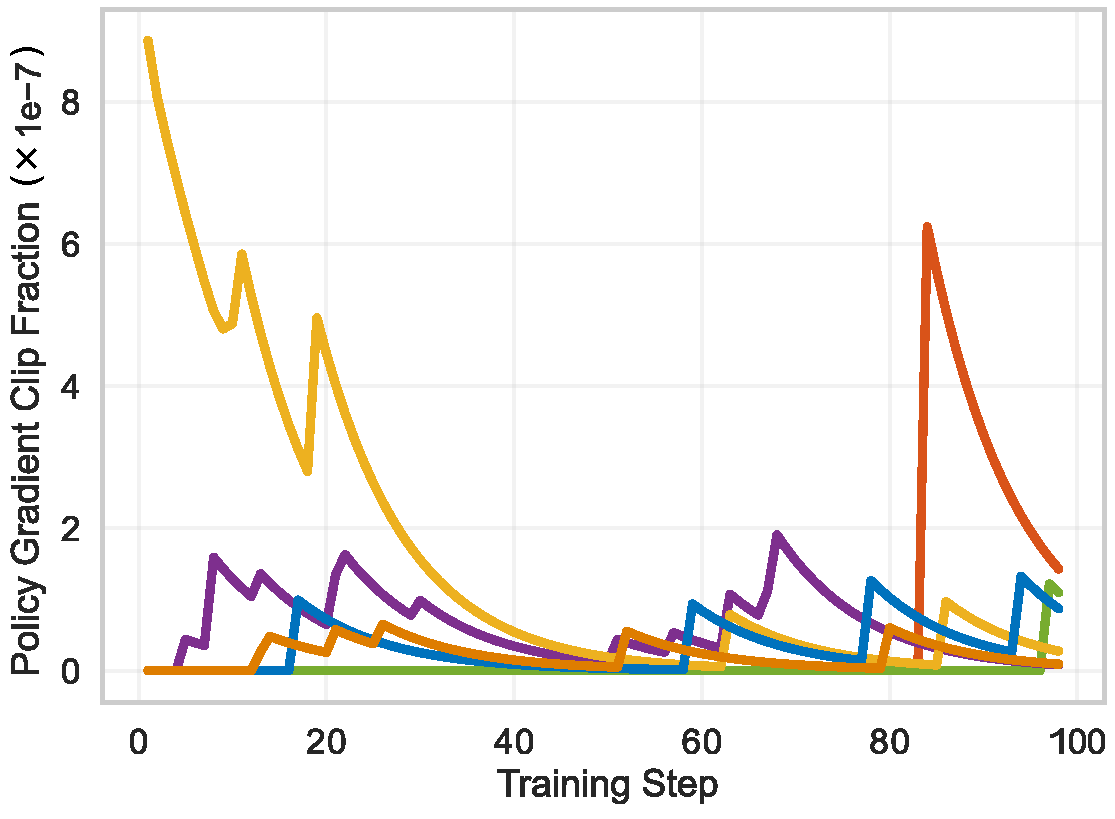
\includegraphics[width=\linewidth]{figures/off-policy-problem/pg_clipfrac_Qwen2.5-Math-1.5B.pdf}
    \caption{Clip Fraction Surge}
    \label{fig: off_policy_pg_clipfrac}
  \end{subfigure}
  \begin{subfigure}[b]{0.28\textwidth}
    \centering
    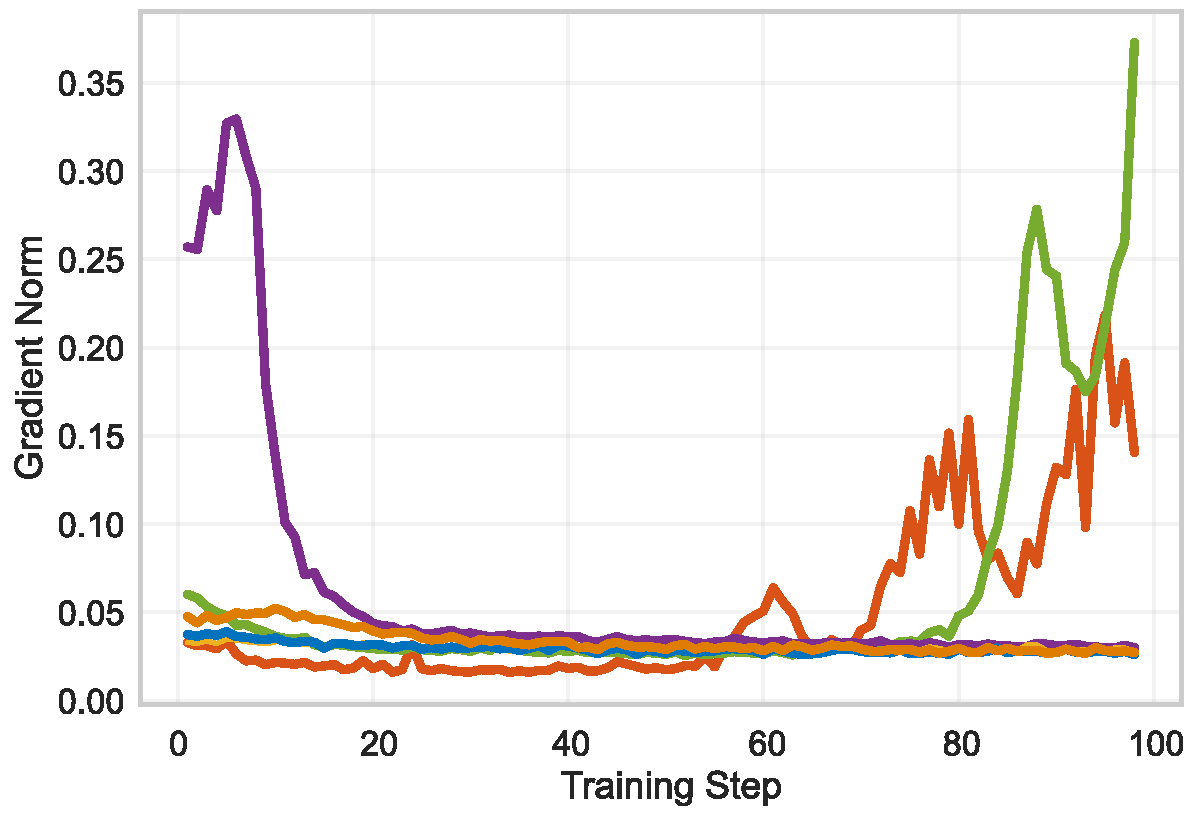
\includegraphics[width=\linewidth]{figures/off-policy-problem/grad_norm_Qwen2.5-Math-1.5B.pdf}
    \caption{Gradient Norm Surge.}
    \label{fig: off_policy_grad_norm}
  \end{subfigure}
   \begin{subfigure}[b]{0.27\textwidth}
    \centering
    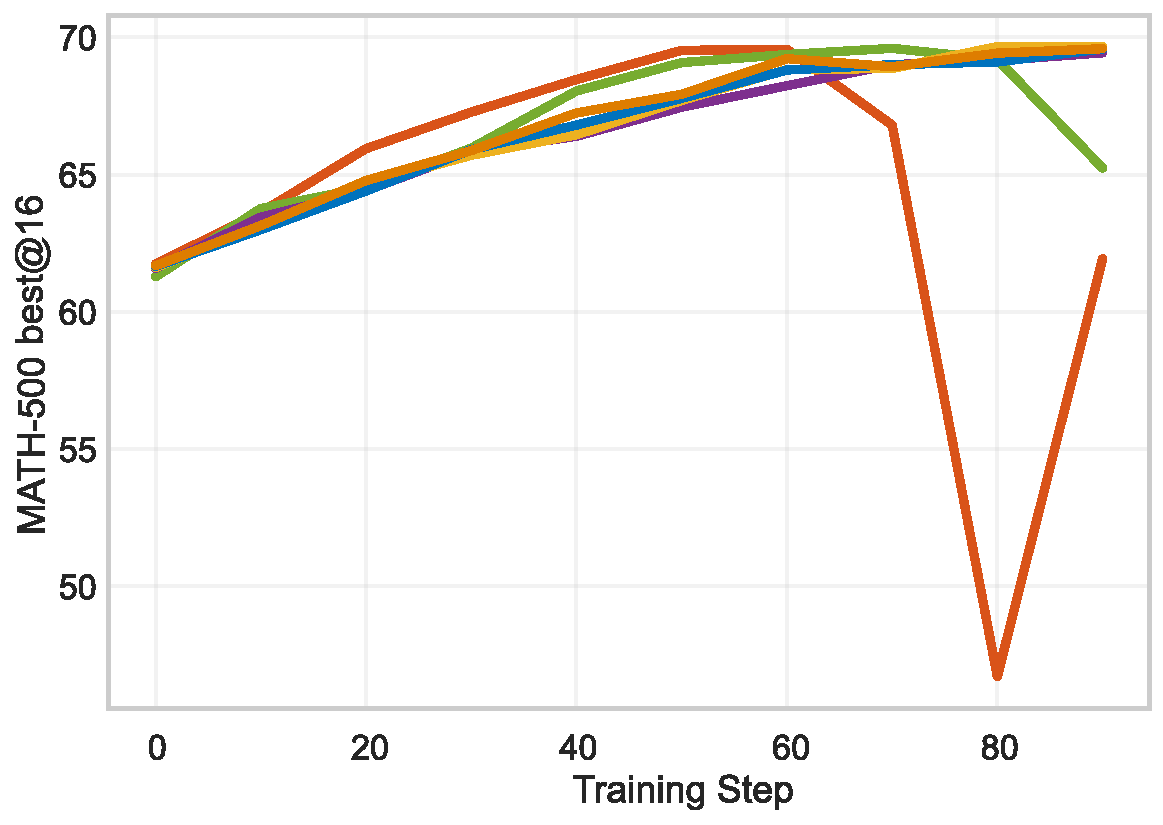
\includegraphics[width=\linewidth]{figures/off-policy-problem/best_at_16_Qwen2.5-Math-1.5B.pdf}
    \caption{Drastic Best@16 Drop}
     \label{fig: off_policy_best_at_16}
  \end{subfigure}
  \begin{subfigure}[t]{0.1\textwidth}
    \centering
    \vspace{-2.5cm}
    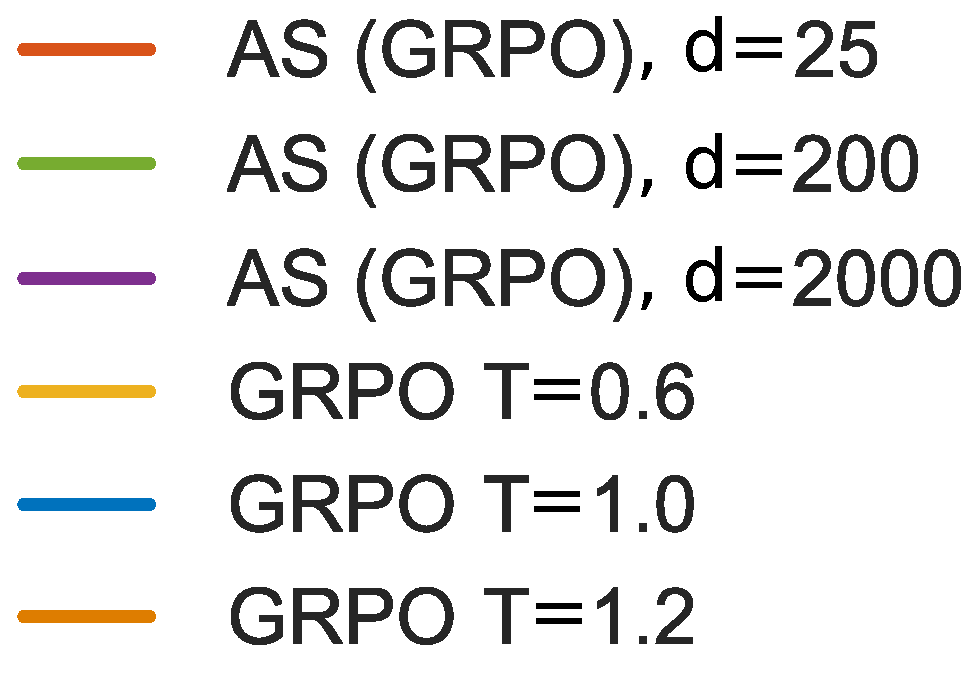
\includegraphics[width=\linewidth]{figures/off-policy-problem/legend-fig3.pdf}
  \end{subfigure}
  \caption{Off-policy samples bring training instability. The base model is Qwen2.5-Math-1.5B.}
  \label{fig:optim_failure_for_as_offpolicy}
\end{figure}

Noted that this off-policy phenomenon widely exists for any efficient sampling framework \citep{yao2025offpolicy} and sampling strategy (for instance, when applying best-of-$n$ sampling \citep{xiong2025minimalist} or filtering out responses \citep{shrivastava2025sample}, the underlying distribution of responses is implicitly altered). To be more precise, we take the policy gradient loss as an example:
\begin{align*}
\E_{x \sim \mathcal{D},y{\sim} \mathbin{\color{red}\pi^{\text{sampling}}_{\theta_{\text{old}}}(\cdot\mid x)}}
\left[\frac{\pi_{\theta}(y\mid x)}{\pi_{\theta_{\text{old}}}(y\mid x)}A(y;x)\right] 
=\E_{x \sim \mathcal{D},y{\sim} \mathbin{\pi_{\theta_{\text{old}}}(\cdot\mid x)}}\left[{\color{red}\frac{\pi^{\text{sampling}}_{\theta_{\text{old}}}(y\mid x)}{\pi_{\theta_{\text{old}}}(y\mid x)}}\times\frac{\pi_{\theta}(y\mid x)}{\pi_{\theta_{\text{old}}}(y\mid x)}A(y;x)\right],
\end{align*}
where $\pi^{\text{sampling}}_{\theta_{\text{old}}}(\cdot\mid x)$ represents the underlying sampling distribution. 
In such case, an extra weight is implicitly added to each response in addition to its advantage $A(y;x)$.

This extra weight can significantly inflate the variance of the policy gradient, posing a stability challenge that our proposed \alg needs to mitigate.
To quantify this effect in our proposed \alg, we now analyze such variance under a standard, fixed \textbf{temperature sampling}.

% \paragraph{Temperature Sampling.} 
We use $\tau=1$ to define a policy $\pi$ and consider the effect of $\tau$ on the variance of the gradient estimator. We reduce the problem to analyzing the variance inflation factor
\begin{equation}
\label{eq:variance-inflation-factor}
\mathbb{E}_{y\sim\pi(\cdot\mid x;\tau)}\left[\frac{\pi(y\mid x;1)^2}{\pi(y\mid x;\tau)^2}\right].
\end{equation}
We begin with one-token case. Let $o_i$ denote the $i$th token in the vocabulary $V$ and $h_i$ is its logit. Then \eqref{eq:variance-inflation-factor} can be rewritten as
\begin{align*}
    \sum_{i=1}^{|V|}\frac{h_i/(\sum_{j=1}^{|V|} h_j)}{h^{1/\tau}_i/(\sum_{j=1}^{|V|} h^{1/\tau}_j)}\times\frac{h_i}{\sum_{j=1}^{|V|} h_j}
    = \frac{\sum_{i=1}^{|V|} h_i^{2-1/\tau}\sum_{i=1}^{|V|} h^{1/\tau}_i}{\left(\sum_{i=1}^{|V|} h_i\right)^2}
\end{align*}

\begin{proposition}
Suppose $h_i\in[0,1]$ for all $i\in V$.
$\sum_{i=1}^{|V|} h_i^{2-1/\tau}\sum_{i=1}^{|V|} h^{1/\tau}_i$ is decreasing when $\tau\le1$ and increasing when $\tau\ge1$, which implies it has a global minimum at $\tau=1$.
\end{proposition}
\begin{proof}
Let $x=1/\tau$. We define 
\[
f(x)=\log\left(\sum_{i=1}^{|V|} h_i^{2-x}\right)+\log\left(\sum_{i=1}^{|V|} h^{x}_i\right).
\]
Its derivative is
\[
f'(x)=\frac{-\sum_{i=1}^{|V|} h_i^{2-x}\log h_i}{\sum_{i=1}^{|V|} h_i^{2-x}}
+\frac{\sum_{i=1}^{|V|} h_i^{x}\log h_i}{\sum_{i=1}^{|V|} h_i^{x}}.
\]
To analyze the sign of $f'(x)$, we define a helper function $g(x) = \frac{\sum_{i=1}^{|V|} h_i^{x}\log h_i}{\sum_{i=1}^{|V|} h_i^{x}}$. Then, $f'(x)=g(x)-g(2-x)$ and its sign depends on whether $g(x)$ is greater than, less than, or equal to $g(2-x)$. We take a look at derivative of $g$:
\[
g'(x) = \frac{\left(\sum_{i=1}^{|V|} h_i^{x}(\log h_i)^2\right) \left(\sum_{i=1}^{|V|} h_i^{x}\right) - \left(\sum_{i=1}^{|V|} h_i^{x}\log h_i\right)^2}{\left(\sum_{i=1}^{|V|} h_i^{x}\right)^2}\ge0.
\]
Hence, $g$ is an increasing function and
\begin{equation*}
\begin{cases}
~f'(x)=g(x)-g(2-x)\ge0,~~\mathrm{when}~x\ge1\\
~f'(x)=g(x)-g(2-x)=0,~~\mathrm{when}~x=1\\
~f'(x)=g(x)-g(2-x)\le0,~~\mathrm{when}~x\le1.
\end{cases}
\end{equation*}
Accordingly, $f$ is increasing when $x\ge1$ and is decreasing when $x\le1$. Then the proposition easily follows.
\end{proof}

The same conclusion can be proved for multiple-token sequence by induction. Therefore, we get that
when the temperature is far from 1, the off-policy issue could be severe and lead to large variance of the gradient estimator. 


\subsection{Truncated Importance Sampling Ratio Correction}
\label{subsec:tis-correction}
% Such techniques can extensively be applied to prevent extreme likelihood ratios and the resulting huge gradients, thereby enhancing training stability. 
To cancel such bias, an importance sampling ratio can be introduced~\citep{hilton2022batch,yao2025offpolicy}:
% Such bias can be corrected by introducing an importance sampling ratio:
\begin{align*}
\E_{x \sim \mathcal{D},y{\sim} \mathbin{\pi_{\theta_{\text{old}}}(\cdot\mid x)}}\left[\frac{\pi_{\theta}(y\mid x)}{\pi_{\theta_{\text{old}}}(y\mid x)}A(y;x)\right]
=
\E_{x \sim \mathcal{D},y{\sim} \mathbin{\color{red}\pi^{\text{sampling}}_{\theta_{\text{old}}}(\cdot\mid x)}}
\left[{\color{red}\frac{\pi_{\theta_{\text{old}}}(y\mid x)}{\pi^{\text{sampling}}_{\theta_{\text{old}}}(y\mid x)}}\times\frac{\pi_{\theta}(y\mid x)}{\pi_{\theta_{\text{old}}}(y\mid x)}A(y;x)\right]. 
\end{align*}
To further prevent negative effects by the extreme likelihood ratios and boost training stability, we truncate the likelihood ratio with an upper bound. That is, \emph{truncated importance sampling} technique \citep{heckman1998matching}. Taking the vanilla policy gradient loss as an example, the modified loss for EAD is as follows:
\begin{equation*}
\label{eq:tis-pg}
\E_{x \sim \mathcal{D},y{\sim}{\pi^{\text{EAD}}_{\theta_{\text{old}}}(\cdot\mid x)}}
\left[{\color{blue}\min\left(\frac{\pi_{\theta_{\text{old}}}(y\mid x)}{\pi^{\text{EAD}}_{\theta_{\text{old}}}(y\mid x)},\varepsilon\right)}\frac{\pi_{\theta}(y\mid x)}{\pi_{\theta_{\text{old}}}(y\mid x)}A(y;x)\right].
\end{equation*}

% ===== BEGIN COLM REBUTTAL EDIT: TIS specifics + bias note =====
\colmedit{%
\paragraph{Practical choices and bias-variance trade-off.}
We use a per-sequence truncation threshold $\varepsilon = 2.0$ following~\citet{yao2025offpolicy}; this is the same value used for the fixed-temperature baseline whenever it also relies on vLLM-side floating-point corrections. The ratio is computed at the sequence level on the same sequences used for the policy update, and it is evaluated under the reference distribution $\pi_{\theta_{\text{old}}}$, not under the parameters being optimized, so the corresponding term has no gradient contribution.

Truncation introduces a deterministic downward bias on samples whose ratio exceeds $\varepsilon$, but in exchange it bounds the variance of the gradient estimator by $O(\varepsilon^2)$ per sample. For \alg with $\tau_{\min} \geq 0.1$ and $\tau_{\max} \leq 1.2$, we empirically find that fewer than $1\%$ of sequences hit the truncation threshold (\cref{fig: off_policy_pg_clipfrac}), so the bias is small in practice. Setting $\varepsilon \to \infty$ recovers vanilla importance sampling (unbiased but with the empirically destabilising variance shown in \cref{fig:optim_failure_for_as_offpolicy}); setting $\varepsilon \to 1$ recovers the naive uncorrected estimator. Our default $\varepsilon = 2$ sits well in the middle of this trade-off.
}
% ===== END COLM REBUTTAL EDIT =====

% One subtle yet troublesome drawback of RLVR with \algname is that it simultaneously introduces the \emph{off-policy} problem, which might cause training to fail (See \cref{fig:optim_failure_for_as_offpolicy}). This issue arises from the mismatch between the distribution generating the responses and the distribution being optimized. 
% To cancel such bias while guarantee training robustness, we add \emph{truncated importance sampling} technique \citep{heckman1998matching}. Taking the vanilla policy gradient loss as an example, the modified loss is as follows:
% \begin{equation}
% \label{eq:tis-pg}
% \E_{x \sim \mathcal{D},y{\sim}{\pi^{\text{EAD}}_{\theta_{\text{old}}}(\cdot\mid x)}}
% \left[{\color{blue}\min\left(\frac{\pi_{\theta_{\text{old}}}(y\mid x)}{\pi^{\text{EAD}}_{\theta_{\text{old}}}(y\mid x)},\varepsilon\right)}\frac{\pi_{\theta}(y\mid x)}{\pi_{\theta_{\text{old}}}(y\mid x)}A(y;x)\right].
% \end{equation}
% In particular, we pre-specify $\varepsilon=2$.


% \section{Higher Temperature Increases Entropy}
% \label{app: temperature_and_entropy}
\newpage
% \section{Additional Experimental Results}
% % \begin{wrapfigure}{r}{0.43\textwidth}
% % \vspace{-0.5in}
% \begin{figure}[h!]
%     \centering
%     
\includegraphics[width=0.75\linewidth]{iclr2026/figures/reverse_annealing/best_at_16_Qwen2.5-Math-1.5B-new.pdf}
%     % \vspace{-0.25in}
%     \caption{Reverse Annealing ablation experiment results. The reverse schedule fails to surpass normal temperature sampling, confirming that an annealing (decreasing) schedule is essential for performance gains.} 
%     \label{fig: reverse_annealing}
%     % \vspace{-0.7in}
% \end{figure}
% % \end{wrapfigure}

% \begin{figure}[ht!]
%      \centering
%      \begin{subfigure}[h]{0.49\textwidth}
%          \centering
%          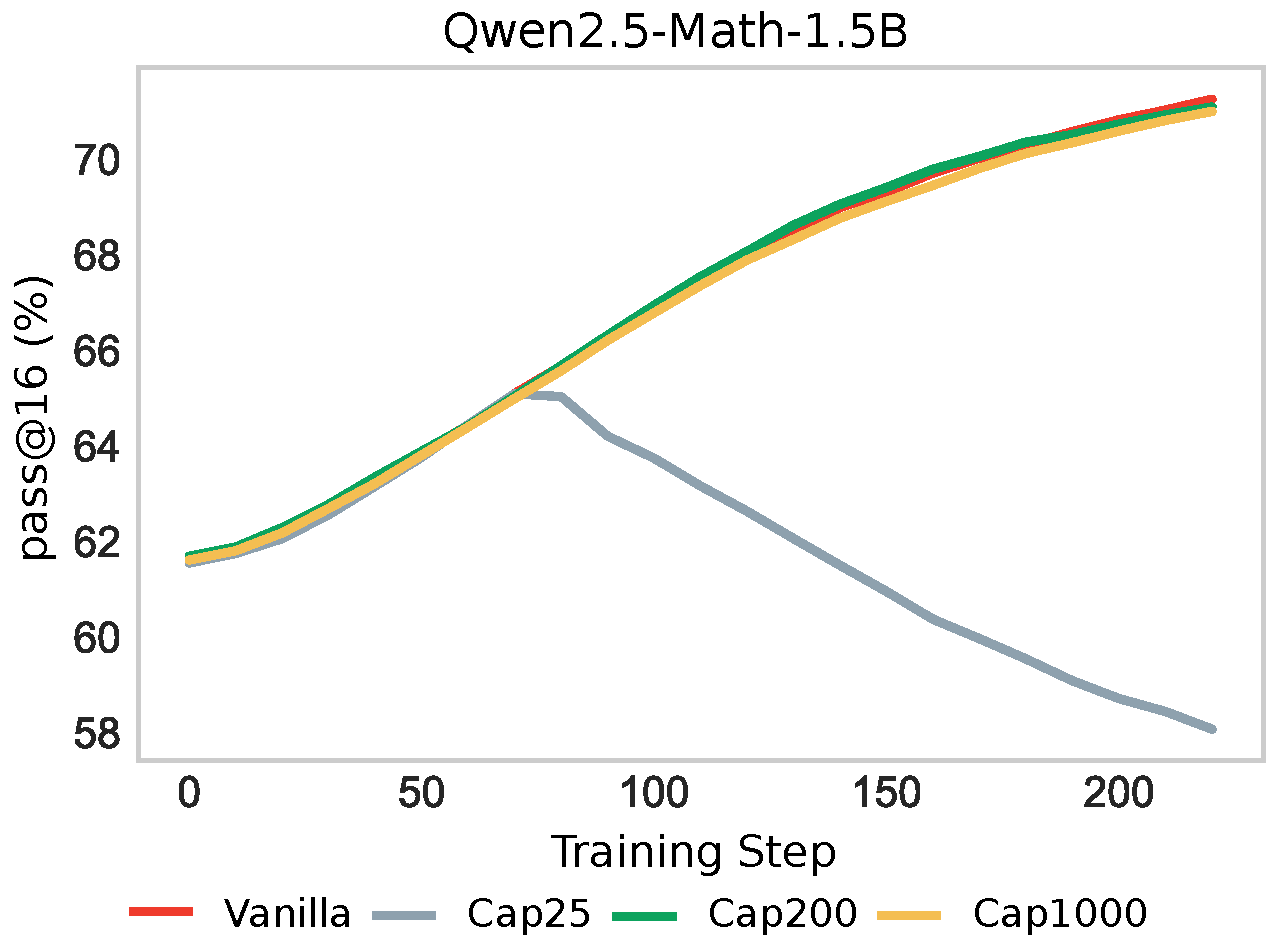
\includegraphics[width=\textwidth]{iclr2026/figures/ablation_cap/best_at_16_Qwen2.5-Math-1.5B-new.pdf}
%          \caption{Decay cap $d_{\max}$.}
%          \label{fig: ablation_cap}
%      \end{subfigure}
%      \begin{subfigure}[h]{0.49\textwidth}
%          \centering
%          
\includegraphics[width=\textwidth]{iclr2026/figures/ablation_growth_factor_and_decay_freq_init/best_at_16_Qwen2.5-Math-1.5B-new.pdf}
%          \caption{Growth factor $\alpha$ and initial decay $d_0$.}
%          \label{fig: ablation_growth_factor_and_decay_freq_init}
%      \end{subfigure}
% \vspace{-0.1in}
% \caption{Ablation on hyperparameter sensitivity. \textbf{Left:} Ablation on decay cap $d_{\max}$. ``Vanilla'' denotes EAD with the default $d_{\max}=40,000$. Setting $d_{\max}=25$ (where $d_0=25$) mimics a fixed temperature schedule (effectively $\alpha=0$), leading to performance drops as the schedule fails to adapt to longer responses. \alg remains robust provided $d_{\max}$ allows for smooth temperature reduction (e.g., $d_{\max} \ge 200$). \textbf{Right:} Ablation on growth factor $\alpha$ and initial decay $d_0$. With a small $d_0$, a positive growth factor ($\alpha > 0$) is required to adapt to increasing response lengths and maintain a smooth intra-sequence schedule. While a large $d_0$ ensures smoothness even with $\alpha=0$, it limits exploration, resulting in lower learning efficiency.}
% \label{fig:hyper-parameter-sensitivity}
% \end{figure}

\newpage
\section{Ablation Study: Hyperparameter Sensitivity and Scheduling Effects}
\label{app:ablation_details}

\shortparagraph{Hyperparameter Sensitivity.} 
We conduct an ablation study on the decay cap $d_{\max}$ and the growth factor $\alpha$. As shown in \cref{fig: ablation_cap}, \alg is robust to a wide range of $d_{\max}$ values, provided the cap is sufficiently large to ensure a smooth annealing schedule. Conversely, a very small cap (e.g., $d_0=d_{\max}=25$) approximates a fixed schedule (equivalent to $\alpha=0$ throughout training). This setting causes an abrupt performance drop, likely because the model cannot adapt to the increasing response lengths during training (see \cref{app: increased_length}). Alternatively, using a large initial $d_0$ yields a smooth schedule even with $\alpha=0$. However, while training remains stable, performance improves slowly due to overly conservative exploration, as shown in \cref{fig: ablation_growth_factor_and_decay_freq_init}.

\shortparagraph{Intra-Sequence vs.\ Training-Step Scheduling.}
A natural question is whether the gains come from the \emph{intra-sequence} annealing or merely from changing the effective temperature across training steps (via the global-step-aware decay rate). The ablation with $d_0 = d_{\max} = 25$ (\cref{fig: ablation_cap}) isolates this: it retains the intra-sequence schedule but removes the training-step adaptation, and still outperforms the best fixed-temperature baseline, confirming that the within-sequence temperature schedule is the primary driver. The global-step-aware component provides further gains by keeping the schedule well-calibrated as response lengths grow.

\begin{figure}[h!]
     \centering
     \begin{subfigure}[h]{0.49\textwidth}
         \centering
         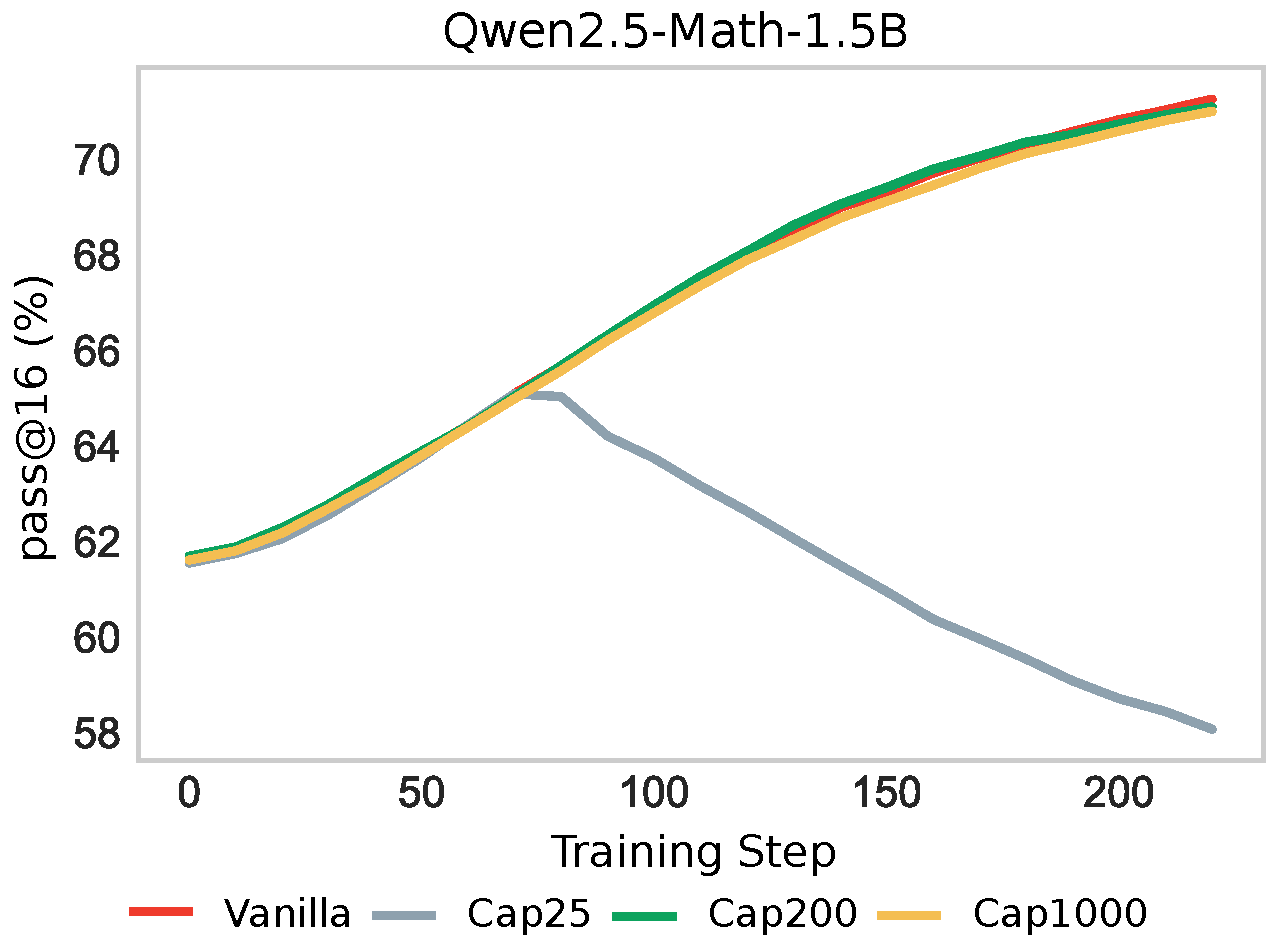
\includegraphics[width=\textwidth]{figures/ablation-cap.pdf}
         \caption{Decay cap $d_{\max}$.}
         \label{fig: ablation_cap}
     \end{subfigure}
     \begin{subfigure}[h]{0.49\textwidth}
         \centering
         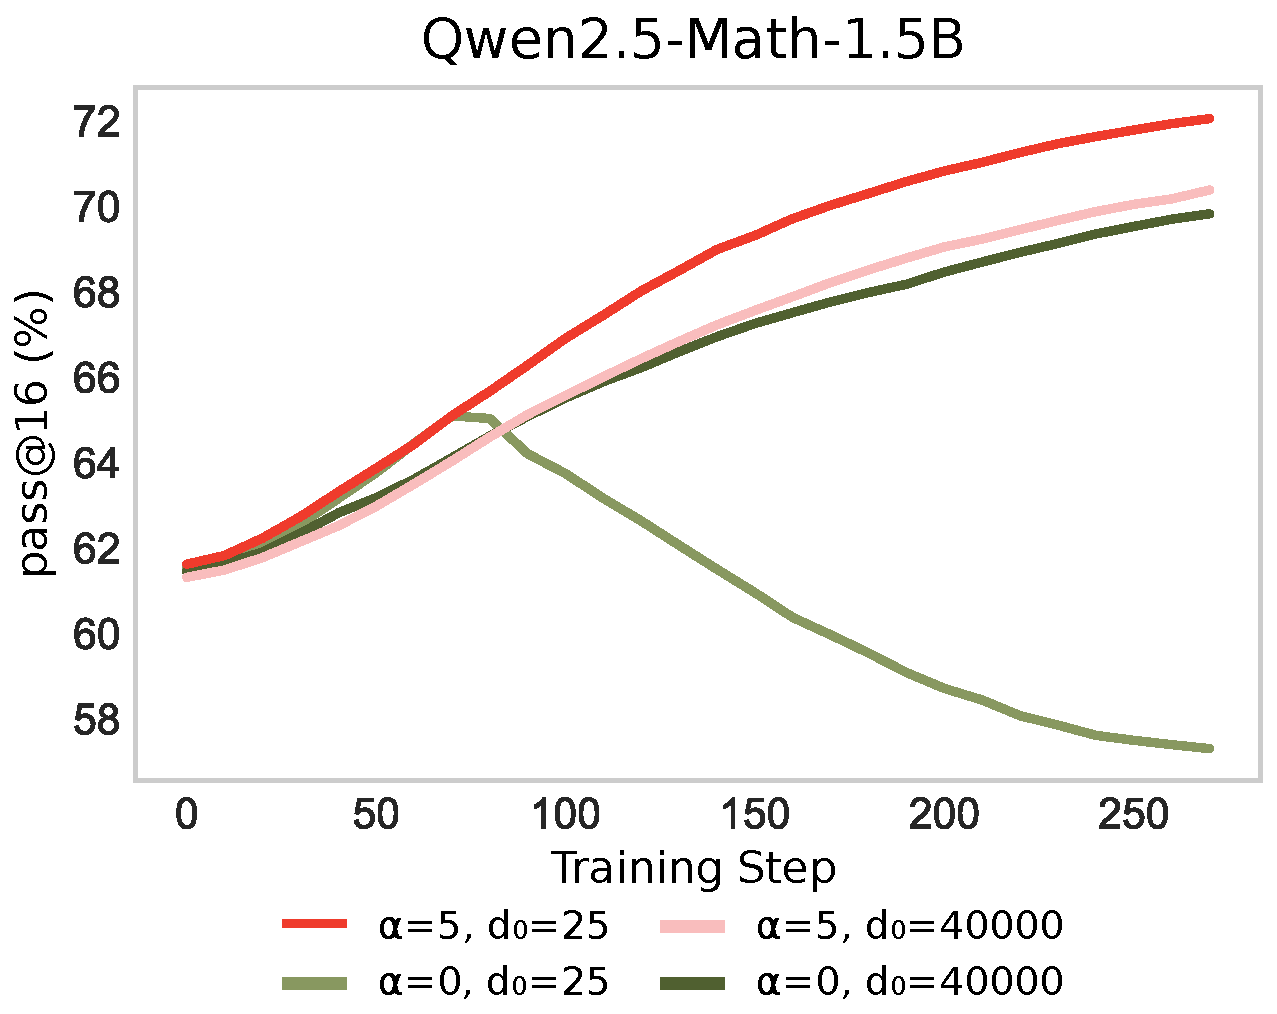
\includegraphics[width=\textwidth]{figures/ablation-growth-factor-and-decay-freq-init.pdf}
         \caption{Growth factor $\alpha$ and initial decay $d_0$.}
         \label{fig: ablation_growth_factor_and_decay_freq_init}
     \end{subfigure}
\caption{Ablation on hyperparameter sensitivity. \textbf{Left:} Ablation on decay cap $d_{\max}$. ``Vanilla'' denotes EAD with the default $d_{\max}=40000$. Setting $d_{\max}=25$ (where $d_0=25$) mimics a fixed temperature schedule (effectively $\alpha=0$), leading to performance drops as the schedule fails to adapt to longer responses. \alg remains robust provided $d_{\max}$ allows for smooth temperature reduction (e.g., $d_{\max} \ge 200$). \textbf{Right:} Ablation on growth factor $\alpha$ and initial decay $d_0$. With a small $d_0$, a positive growth factor ($\alpha > 0$) is required to adapt to increasing response lengths and maintain a smooth intra-sequence schedule. While a large $d_0$ ensures smoothness even with $\alpha=0$, it limits exploration, resulting in lower learning efficiency.}
\label{fig:hyper-parameter-sensitivity}
\end{figure}

\section{Stress Test: DAPO-17K Recipe for AIME24}
\label{app:stress_test}
To verify the effectiveness of \alg on realistic mathematical reasoning tasks, we stress-test it using the DAPO recipe~\citep{yu2025dapo}, training on DAPO-17k and evaluating on the challenging AIME 2024 benchmark. To accommodate GPU memory constraints, we utilize the Qwen-3-8B-Base~\citep{yang2025qwen3} model (instead of 32B) and reduce the maximum response length from 20480 to 8192. We set $d_0=500$ and $d_{\max}=40000$, and vary $\alpha \in \{5, 50\}$. As shown in \cref{fig: aime24}, \alg achieves improved learning efficiency and consistently outperforms the standard temperature sampling baseline. We note that this experiment was conducted under reduced compute (8B model, shorter max length) and was not trained to full convergence; the results primarily demonstrate that \alg accelerates learning, with the final performance ceiling under full-scale training left for future work.

\begin{figure}[h!]
    \centering
    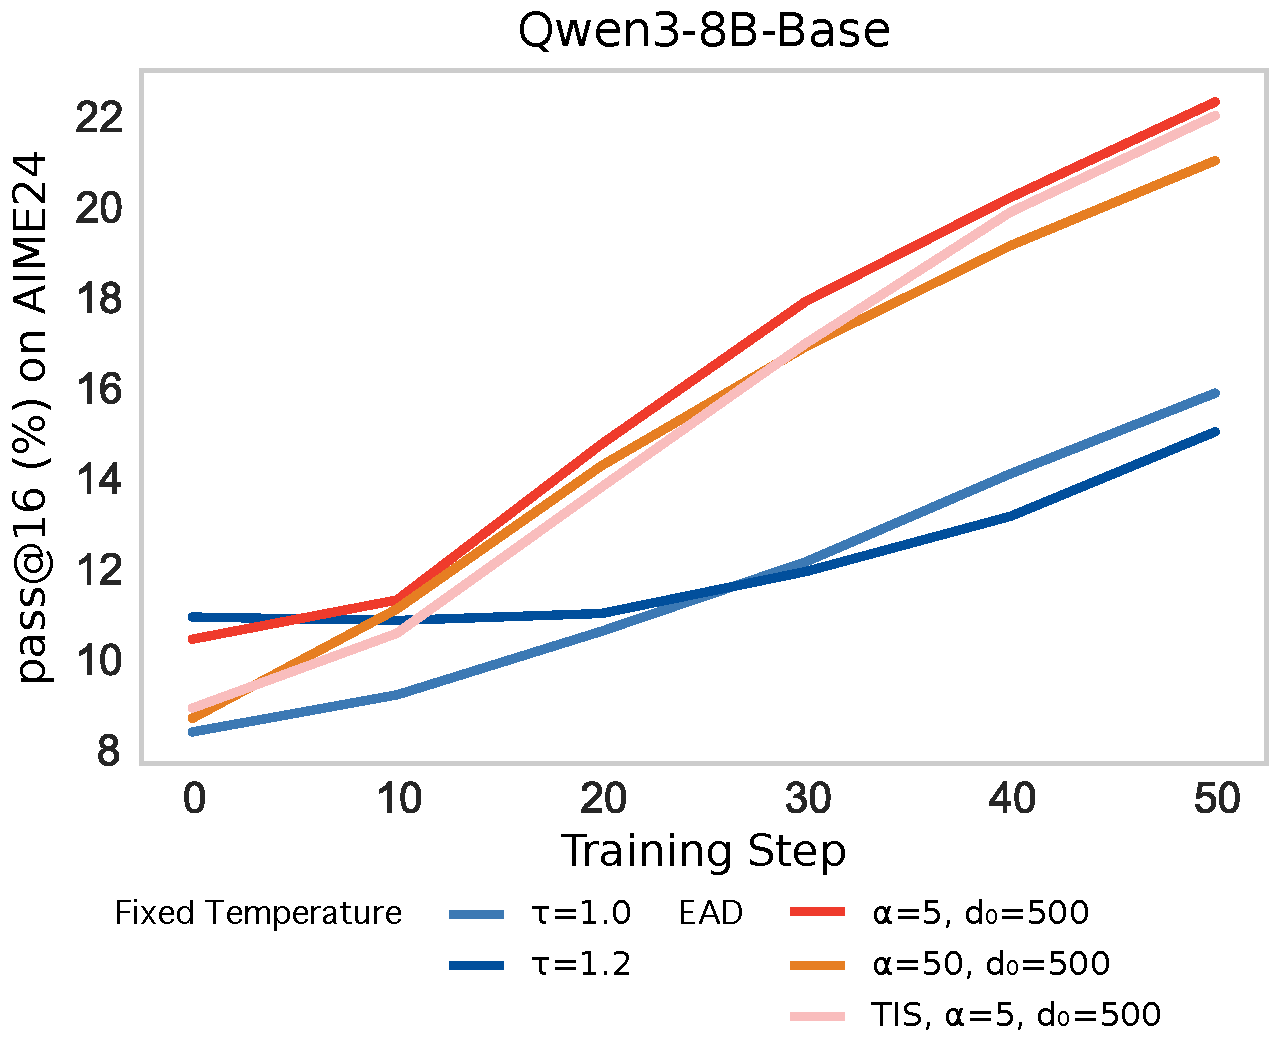
\includegraphics[width=0.66\linewidth]{figures/aime24.pdf}
    \caption{Stress-test of \alg using the DAPO recipe on AIME24. \alg outperforms the temperature sampling baseline across various hyperparameter setups.} 
    \label{fig: aime24}
\end{figure}

\newpage
\section{Connection to Simulated Annealing}
\label{app:simulated_annealing}
Simulated Annealing (SA) is a probabilistic optimization technique inspired by annealing in metallurgy, designed to find the global optimum in a large search space \citep{kirkpatrick1983optimization, bertsimas1993simulated}. The core principle involves a temperature parameter that controls the probability of accepting suboptimal states. Initially, a high temperature allows the search to escape local minima by exploring broadly (exploration). As the temperature gradually decreases, the algorithm increasingly favors better states, converging towards a high-quality solution (exploitation).
This ``coarse-to-fine'' search dynamic, where high temperatures establish a solution's general structure and low temperatures refine its details, strongly parallels the generative process of LLMs \citep{yang2025alignment}. SA has been adapted in various machine learning contexts to manage the exploration-exploitation trade-off, including recent applications in graph optimization~\citep{liu2021simulated}, text editing \citep{zhang2024edt}, non-autoregressive generation \citep{israel2025enabling}, and efficient Best-of-N sampling \citep{manvi2024adaptive}. However, these prior applications invariably apply a single, uniform temperature across all positions in a generated sequence. This approach fails to account for the heterogeneous roles of tokens at different positions \citep{wang2025beyond}. Our work departs from this convention. To the best of our knowledge, we are the first to introduce an \textbf{intra-sequence annealed temperature} schedule, where the temperature varies dynamically within the generation of a single sequence. This novel approach allows for more nuanced control over exploration and leads to significant performance gains in RLVR.

\newpage
\section{Proof of Temperature-Entropy Relationship}
\label{app:entropy_proof}

% \newtheorem{proposition}{Proposition}
\begin{proposition}
The entropy of the softmax distribution is a non-decreasing function of the temperature $\tau > 0$.
\end{proposition}

\begin{proof}
The strategy is to show that the entropy $H$ is a non-increasing function of the inverse temperature $\beta = 1/\tau > 0$.
The probability of sampling token $v$ with temperature $\tau$ is given by the policy $\pi_\theta$. For simplicity in the derivation, we denote this probability as $p_v(\tau)$:
\[
p_v(\tau) \triangleq \pi_\theta(y_t=v \mid [x, y_{<t}]; \tau)
\]
% = \frac{\exp(h_v / \tau)}{\sum_{v' \in V} \exp(h_{v'} / \tau)}.$

Let $h_v$ be the logit for a token $v$ in the vocabulary $V$. The probability of a token as a function of $\beta$ is given by:
\[
p_v(\beta) = \frac{\exp(\beta h_v)}{\sum_{v' \in V} \exp(\beta h_{v'})} \triangleq \frac{\exp(\beta h_v)}{Z(\beta)},
\]
where $Z(\beta)$ is the partition function. The entropy, as a function of $\beta$, is:
\[
H(\beta) = -\sum_{v \in V} p_v(\beta) \log p_v(\beta).
\]
We can rewrite the entropy by substituting $\log p_v(\beta) = \beta h_v - \log Z(\beta)$:
\begin{align*}
H(\beta) &= -\sum_{v \in V} p_v(\beta) (\beta h_v - \log Z(\beta)) \\
&= \log Z(\beta) \left(\sum_{v \in V} p_v(\beta)\right) - \beta \sum_{v \in V} h_v p_v(\beta) \\
&= \log Z(\beta) - \beta \cdot \mathbb{E}_{v \sim p(\beta)}[h_v].
\end{align*}
Now, we differentiate $H(\beta)$ with respect to $\beta$. Let $\bar{h}(\beta) = \mathbb{E}[h_v]$.
\[
\frac{dH}{d\beta} = \frac{d}{d\beta}(\log Z(\beta)) - \frac{d}{d\beta}(\beta \bar{h}(\beta)).
\]
First, we find the derivative of the log-partition function:
\[
\frac{d}{d\beta}(\log Z(\beta)) = \frac{Z'(\beta)}{Z(\beta)} = \frac{\sum_v h_v \exp(\beta h_v)}{Z(\beta)} = \sum_v h_v p_v(\beta) = \bar{h}(\beta).
\]
Next, we use the product rule for the second term:
\[
\frac{d}{d\beta}(\beta \bar{h}(\beta)) = \bar{h}(\beta) + \beta \frac{d\bar{h}}{d\beta}.
\]
Combining these gives:
\[
\frac{dH}{d\beta} = \bar{h}(\beta) - \left(\bar{h}(\beta) + \beta \frac{d\bar{h}}{d\beta}\right) = -\beta \frac{d\bar{h}}{d\beta}.
\]
The derivative $\frac{d\bar{h}}{d\beta}$ is the variance of the logits. We can show this by differentiating $\bar{h}(\beta)$:
\begin{align*}
\frac{d\bar{h}}{d\beta} &= \frac{d}{d\beta}\left( \frac{\sum_v h_v \exp(\beta h_v)}{Z(\beta)} \right) \\
&= \frac{(\sum_v h_v^2 \exp(\beta h_v))Z(\beta) - (\sum_v h_v \exp(\beta h_v))Z'(\beta)}{Z(\beta)^2} \\
&= \sum_v h_v^2 p_v(\beta) - \left(\sum_v h_v p_v(\beta)\right)\left(\frac{Z'(\beta)}{Z(\beta)}\right) \\
&= \mathbb{E}[h^2] - (\mathbb{E}[h])^2 = \mathrm{Var}_{v \sim p(\beta)}(h_v).
\end{align*}
Substituting this back, we arrive at the final expression for the derivative of entropy:
\[
\frac{dH}{d\beta} = -\beta \cdot \mathrm{Var}_{v \sim p(\beta)}(h_v).
\]
By definition, the temperature $\tau > 0$, so the inverse temperature $\beta > 0$. The variance of any random variable is non-negative. This can be formally shown using \textbf{Jensen's inequality}: for the convex function $\phi(x)=x^2$, we have $\mathbb{E}[\phi(h)] \ge \phi(\mathbb{E}[h])$, which means $\mathbb{E}[h^2] \ge (\mathbb{E}[h])^2$, and thus $\mathrm{Var}(h) \ge 0$.

Therefore, the derivative of entropy with respect to $\beta$ is non-positive:
\[
\frac{dH}{d\beta} = \underbrace{-\beta}_{\le 0} \cdot \underbrace{\mathrm{Var}(h_v)}_{\ge 0} \le 0.
\]
Since $H(\beta)$ is a non-increasing function of $\beta$, and $\beta$ is inversely proportional to $T$, it follows that $H(\tau)$ must be a non-decreasing function of the temperature $\tau$.
\end{proof}

\section{Increasing Length in RL Training}
\label{app: increased_length}
During RL training, our algorithm (\alg) incentivizes the model to generate longer, more effective reasoning chains for difficult problems, especially for 7B models (\cref{fig: response_length}). While both \alg and temperature sampling initially learn to shorten their responses by shifting from complex code-based solutions to direct mathematical reasoning, their behavior later diverges. The response length from temperature sampling stabilizes, whereas \alg learns to selectively increase reasoning length for harder problems, which boosts final performance. For these experiments, EAD is applied in the DAPO algorithm for sampling rollouts. We use the same training setup as detailed in \cref{sec:experiments}. 

\begin{figure}[h!]
\centering
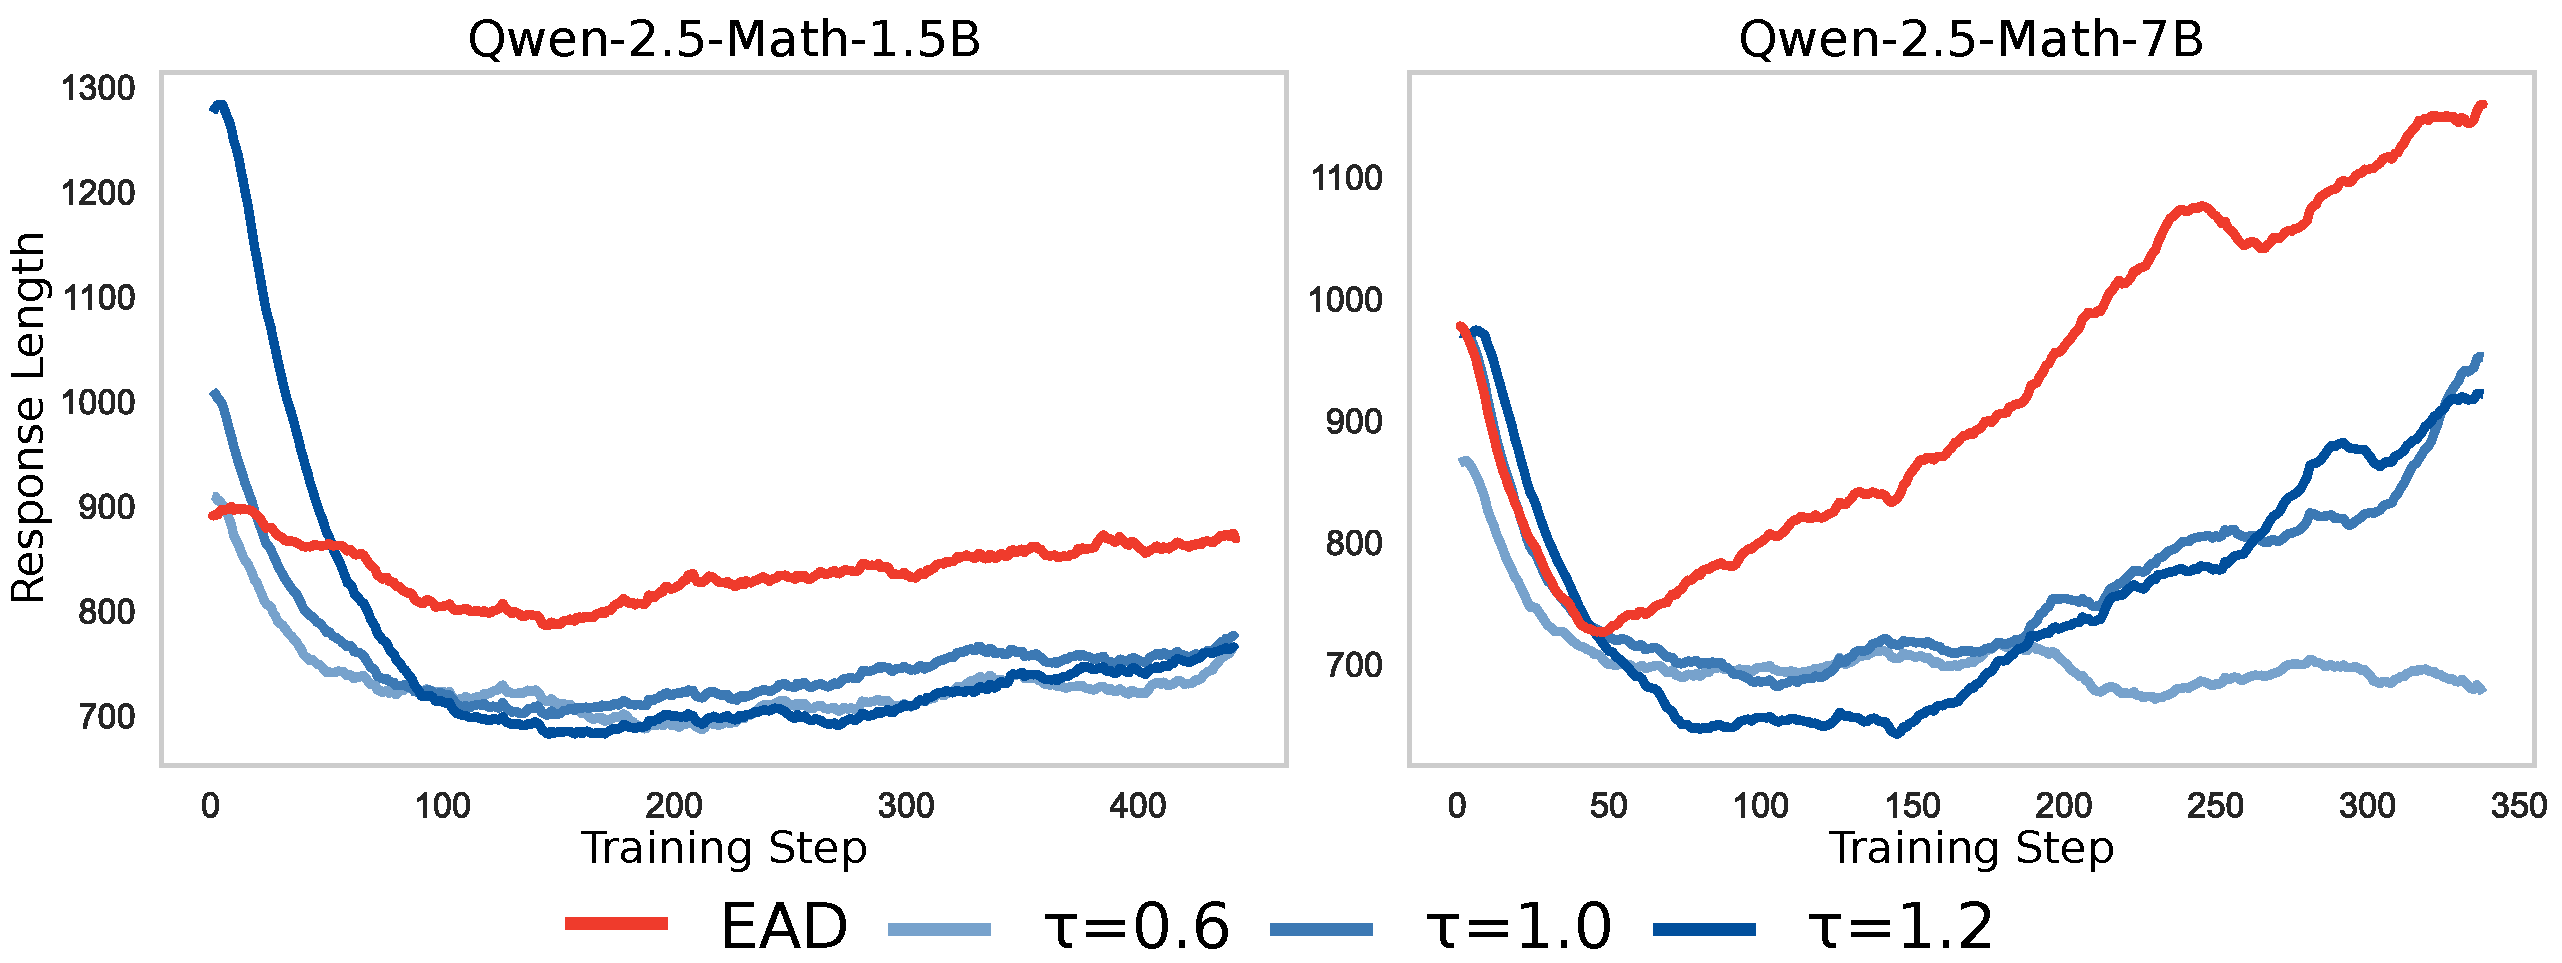
\includegraphics[width=\linewidth]{figures/response-length.pdf}
\caption{Compared with normal temperature sampling, EAD can naturally incentivize the model to generate longer reasoning chains. }
\label{fig: response_length}
\end{figure}

% ===== BEGIN COLM REBUTTAL EDIT: hyperparameter table + selection guide =====
\colmedit{%
\section{\alg Hyperparameter Summary and Selection Guide}
\label{sec:hp}

\paragraph{Defaults used in this paper.}
\Cref{tab:hparam} lists the \alg hyperparameters used in our main experiments. All values were chosen on a small grid over a held-out validation prompt set and then \emph{frozen} across datasets, algorithms (DAPO / GRPO / EntropyMech), and seeds. We did not re-tune them per benchmark.

\begin{table}[h!]
\centering
\small
\begin{tabular}{lccccc}
\toprule
Model family & $\tau_{\max}$ & $\tau_{\min}$ & $d_0$ & $\alpha$ & $d_{\max}$ \\
\midrule
Llama-3.2-1B-Instruct (math)     & 1.2 & 0.1 & 200 & 5 & $4{\times}10^4$ \\
Qwen-2.5-Math-1.5B (math)        & 1.2 & 0.1 & 200 & 5 & $4{\times}10^4$ \\
Qwen-2.5-Math-7B (math)          & 1.2 & 0.6 & 250 & 5 & $4{\times}10^4$ \\
Qwen-3-8B-Base (AIME stress test)& 1.2 & 0.1 & 500 & 5 / 50 & $4{\times}10^4$ \\
\bottomrule
\end{tabular}
\caption{\alg defaults across our experimental settings. The only model-dependent value is $\tau_{\min}$ for the 7B model, where a higher floor avoids over-confident greedy decoding on already-sharp distributions.}
\label{tab:hparam}
\end{table}

\section{Hyperparameter Selection Guide for Practitioners}
\label{sec:hp_guide}
We summarise practical rules of thumb derived from the ablations in
\cref{app:ablation_details,fig:schedule_shapes}:
\begin{itemize}
\item \textbf{$\tau_{\max}$}: pick the highest value that does not noticeably hurt single-sample quality on a small validation set. For our models, $\tau_{\max} \in [1.1, 1.3]$ all worked; the paper uses $1.2$ throughout.
\item \textbf{$\tau_{\min}$}: scales with model sharpness. For 1B-1.5B models, $0.1$ is safe. For 7B+ models with already-sharp next-token distributions, set $\tau_{\min} \approx 0.5\text{--}0.8$ to avoid the schedule collapsing to near-greedy decoding in the late half.
\item \textbf{$d_0$}: roughly the number of tokens you want the schedule to ``stay hot'' at the start of training. We pick $d_0$ so that $\tau_t \geq 1.0$ for the first $\sim 100$ tokens at step 0. Our defaults satisfy this.
\item \textbf{$\alpha$}: the growth factor. The schedule needs to track the response-length increase during training (\cref{app: increased_length}); $\alpha = 5$ (linear growth at one extra ``hot'' token per training step) was sufficient for all our runs.
\item \textbf{$d_{\max}$}: an upper bound that prevents pathological late-training behaviour where the schedule never reaches $\tau_{\min}$. Any value in $[10^3, 10^5]$ gave near-identical performance (\cref{fig: ablation_cap_extended}); we use $4{\times}10^4$.
\item \textbf{$c$}: template-cutoff. Keep $c$ at one to two dozen tokens so that chat-formatting tokens (e.g.\ \texttt{Let's think step by step}) are decoded at standard temperature and do not get pushed off-distribution by $\tau_{\max} > 1$.
\end{itemize}

\section{Schedule-Shape Ablation}
\label{app:schedule_shapes}
\colmnote{Figure to be filled in by the rebuttal run; the recipe is in \texttt{recipe/annealed\_sampling/ablation\_schedule\_shapes\_qwen\_math\_1\_5b.sh}.}

We compare four temperature schedules with identical hyperparameters
$(\tau_{\max},\tau_{\min},d_0,\alpha,d_{\max}) = (1.2, 0.1, 200, 5, 40000)$ but different shapes (cf. \cref{sec: method}):
\begin{enumerate}
\item \textbf{negexp} ($\alg$, default): $\tau_t = \max\{1 + \tau_{\max} - e^{t/d_s},\;\tau_{\min}\}$.
\item \textbf{linear}: $\tau_t = \max\{\tau_{\max} - (\tau_{\max}{-}\tau_{\min})\cdot\frac{t}{20 d_s},\;\tau_{\min}\}$.
\item \textbf{two\_stage}: $\tau_t = \tau_{\max}$ for $t < 10 d_s$, else $\tau_{\min}$.
\item \textbf{mean\_matched}: fixed $\tau$ equal to the time-average of negexp over $[0, 20 d_s]$. This control has the same per-token entropy budget as negexp.
\end{enumerate}

\begin{figure}[h!]
\centering
\fbox{\parbox{0.8\linewidth}{\centering Placeholder for schedule-shape comparison; the recipe is in \texttt{recipe/annealed\_sampling/ablation\_schedule\_shapes\_qwen\_math\_1\_5b.sh}.}}
\caption{Pass@16 over training for four temperature schedules with matched $(\tau_{\max},\tau_{\min},d_0,\alpha,d_{\max})$. The smooth exponential decay (\alg) dominates both the linear and step-function controls as well as the entropy-matched fixed-temperature control, indicating that the gains are driven by the schedule shape and not simply by the entropy budget.}
\label{fig:schedule_shapes}
\end{figure}

\section{Extended $d_{\max}$ Sensitivity}
\label{app:dmax_sensitivity}
\colmnote{Figure to be filled in by the rebuttal run; the recipe is in \texttt{recipe/annealed\_sampling/ablation\_d\_max\_sweep\_qwen\_math\_1\_5b.sh}.}

\begin{figure}[h!]
\centering
\fbox{\parbox{0.8\linewidth}{\centering Placeholder for $d_{\max}$ sweep over $\{200, 1000, 5000, 40000, 200000\}$.}}
\caption{Extended sweep of $d_{\max}$ for Qwen-2.5-Math-1.5B. Performance is stable across two orders of magnitude in $d_{\max}$, complementing the original $\{25, 200\}$ comparison in \cref{fig: ablation_cap}.}
\label{fig: ablation_cap_extended}
\end{figure}

\section{Code-Reasoning Experiments}
\label{app:code_experiments}

\paragraph{Setup.}
We train Qwen-2.5-Coder-1.5B-Instruct~\citep{hui2024qwen2} with GRPO on a 10K-problem subset of PRIME-RL's Eurus-2 code data~\citep{cui2025process}, which contains stdin/stdout test cases for TACO~\citep{li2023taco}, APPS~\citep{hendrycks2021measuring}, and Codeforces problems. Held-out evaluation is on LiveCodeBench release\_v2~\citep{jain2024livecodebench} (stdin/stdout) and HumanEval+~\citep{liu2023evalplus} (function-call). Candidates are executed locally via PRIME-RL's subprocess + \texttt{SIGALRM} timeout path -- no Docker or external sandbox service is required. Full preprocessing and training scripts are in \texttt{recipe/annealed\_sampling/codeRL/}.

\paragraph{Hyperparameters.}
We use the same \alg defaults as the 1.5B math model (\cref{tab:hparam}). The fixed-temperature baselines are swept over $\tau \in \{0.7, 1.0, 1.2\}$.

\paragraph{Results.}
\colmnote{Numbers to be filled in by the rebuttal run.}

\begin{table}[h!]
\centering
\small
\begin{tabular}{lcc}
\toprule
Method & HumanEval+ Pass@1 & LiveCodeBench Pass@1 \\
\midrule
Fixed $\tau = 0.7$ (best baseline) & TBD & TBD \\
Fixed $\tau = 1.0$                 & TBD & TBD \\
Fixed $\tau = 1.2$                 & TBD & TBD \\
\alg (GRPO)                        & TBD & TBD \\
\bottomrule
\end{tabular}
\caption{Code-reasoning results on Qwen-2.5-Coder-1.5B-Instruct after one epoch of RL on Eurus-2-code (10K problems).}
\label{tab:code_results}
\end{table}

We additionally report an inference-only ``Day-0'' comparison on the base model (no RL) in \cref{tab:code_inference_only}, using the same \alg schedule. This isolates the sampling-side contribution from any RL-training dynamics.

\begin{table}[h!]
\centering
\small
\begin{tabular}{lcc}
\toprule
Method & HumanEval+ Pass@8 & LiveCodeBench Pass@8 \\
\midrule
Fixed $\tau = 0.7$ & TBD & TBD \\
Fixed $\tau = 1.0$ & TBD & TBD \\
Fixed $\tau = 1.2$ & TBD & TBD \\
\alg negexp        & TBD & TBD \\
\bottomrule
\end{tabular}
\caption{Inference-only Pass@8 on the off-the-shelf Qwen-2.5-Coder-1.5B-Instruct model (no RL training).}
\label{tab:code_inference_only}
\end{table}
}
% ===== END COLM REBUTTAL EDIT =====
